%!TEX root = skripsi.tex
%-----------------------------------------------------------------------------%
\chapter{\babTiga}
%-----------------------------------------------------------------------------%
Bab ini akan menjelaskan gambaran proses penelitian secara keseluruhan yang terdiri dari \textit{word alignment} korpus paralel, peningkatan kualitas dan evaluasi \textit{word alignment}, pemindahan \textit{sense} dari korpus bahasa Inggris, dan sistem WSD yang akan diimplementasikan.

%-----------------------------------------------------------------------------%
\section{Penjajaran Kata Korpus Paralel}
%-----------------------------------------------------------------------------%
Penjajaran kata pada korpus berbahasa Inggris dan Indonesia menggunakan \textit{tools word alignment} bernama Giza++. \textit{Tool} ini merupakan salah satu \textit{word alignment tools} pada \textit{statistical machine translation} (SMT) yang dapat digunakan untuk memasangkan kata-kata pada dua buah korpus atau lebih. Terdapat beberapa \textit{word alignment tools} lain seperti Berkeley \textit{aligner}, anymalign, dan lain-lain. Proses penyelarasan yang dilakukan dengan Giza++ meliputi tahap-tahap berikut:
\begin{enumerate}
	\item Mempersiapkan kedua buah \textit{file} yaitu korpus bahasa asal dan korpus bahasa tujuan. Kedua \textit{file} ini berpasangan dalam setiap barisnya. Baris pertama dalam \textit{file} pertama berpasangan dengan baris pertama pada \textit{file} kedua sampai akhir baris pada kedua \textit{file}.
	\item Menghasilkan \textit{file} perbendaharaan kata dari kedua bahasa dan \textit{list} indeks perbendaharaan kata pada tiap kalimat yang sudah diselaraskan
	\item Menghasilkan \textit{cooccurence file} dari kosa kata dan pasangan kalimat tersebut
	\item Proses \textit{alignment} yang menghasilkan beberapa macam \textit{output file} 
\end{enumerate}

Terdapat satu buah \textit{output file} Giza++ yang berisi pasangan-pasangan kalimat dengan kata-kata yang sudah diselaraskan dengan translasinya dalam bahasa tujuan. Hasil ini merupakan \textit{best viterbi alignment} menurut Giza++. Pasangan kalimat dengan kata-kata yang sudah diselaraskan mempunyai bentuk seperti contoh berikut:

\begin{itemize}
	\item Dia pergi ke Bandung malam ini
	\item NULL (\{ \}) She (\{ 1 \}) will (\{ \}) go (\{ 2 \}) to (\{ 3 \}) Bandung (\{ 4 \}) tonight (\{ 5 6 \})
\end{itemize}

Setiap kata pada bahasa tujuan akan memiliki angka hasil penyelarasan yang berkorespondensi pada indeks huruf ke-n pada kata di kalimat bahasa tujuan. Pada contoh tersebut "She" dipasangkan dengan kata pertama yaitu "Dia", kata "will" tidak mempunyai pasangan pada kalimat asal, kata "tonight" dipasangkan dengan kata "malam ini". Bila terdapat kata yang dipasangkan pada token khusus (NULL), dapat diartikan bahwa Giza++ menilai bahwa kata tersebut tidak mempunyai pasangan.

%-----------------------------------------------------------------------------%
\section{Evaluasi \textit{Word Alignment}} \label{sec:pembentukanTdanH}
%-----------------------------------------------------------------------------%
\textit{Word alignment} hasil dari \textit{tool} Giza++ dievaluasi dengan menggunakan \textit{anotator} hasil \textit{alignment} dari \textit{anotator} yang akan ditujukan sebagai \textit{gold standard}. Nilai-nilai yang akan dihitung meliputi \textit{precision} (P), \textit{recall} (R), dan F-\textit{score}. Metode evaluasi keseluruhan meliputi:

\begin{enumerate}
	\item Pemilihan \textit{random sampling} sebanyak seratus buah pasangan kalimat
	\item Masing-masing \textit{anotator} memasang-masangkan kata yang tepat pada masing-masing pasangan kalimat, dengan asumsi bahwa anotasi manusia sebagai \textit{gold standard}
	\item Hasil anotasi manusia dan keluaran dari \textit{tool} Giza dibandingkan untuk mendapatkan ketiga nilai P, R, dan F-Score.
\end{enumerate}


%-------%
\section{Peningkatan Kualitas Hasil \textit{Alignment}}
%-----------------------------------------------------------------------------%
Pengumpulan kata-kata dalam bahasa Indonesia dengan setiap pasangannya di bahasa Inggris dilakukan untuk mempersiapkan pemindahan makna kata tersebut. Permasalahan terjadi ketika didapatkan pasangan kata yang tidak benar seperti pada halnya kata "lapangan" dipasangkan dengan kata dalam bahasa inggris \textit{field}, \textit{ground}, \textit{involved}, \textit{job}, \textit{program}, dan beberapa kata lainnya. Untuk meminimalisir penyimpangan \textit{alignment} yang salah, penulis menggunakan hasil \textit{alignment} dengan menukar antara bahasa asal dan bahasa tujuan. Pemanfaatan \textit{bi-directional alignment} ini ditujukan untuk mengurangi kata-kata yang terlampau jauh dari hasil translasi seharusnya. Konsep dasar dari cara bekerja \textit{filter} ini adalah sebagai berikut:

\begin{lstlisting}[language=Python, caption={Word Alignment Enhancement}, label={word-alignment-enhancement}]

dict_id = {}
dict_en = {}

# masukan setiap kosa kata bahasa Indonesia ke dalam dict_id sebagai key dan kumpulan pasangan kata bahasa inggrisnya sebagai value
# proses yang sama dilakukan untuk dict_en dengan kosa kata bahasa Inggris sebagai key dan kumpulan pasangan kata bahasa Indonesia sebagai value
# stop adalah list stopword yang didapat dari korpus nltk

# this section is for filtering which english word that has corresponding indo translation (bidirectional) from Giza output
for indo_word in dict_id.keys():
	if indo_word not in dict_en:
		# filtering so no same translation is entered, answer -> answer, jawaban -> jawaban
		for en_word in dict_id[indo_word].keys():
			if en_word in dict_en and indo_word in dict_en[en_word] and en_word not in stop:
				if indo_word not in final_dictionary:
					final_dictionary[indo_word] = { en_word: dict_en[word_en][word_id] }
				else:
					if en_word not in final_dictionary[indo_word]:
						final_dictionary[indo_word][en_word] = dict_en[word_en][word_id]
\end{lstlisting}

Pada kasus kata \textbf{lingkungan} dari hasil keluaran Giza memiliki pasangan kata:

\begin{enumerate}
	\item environment
	\item environmental
	\item neighborhood
	\item within
	\item environmentally
\end{enumerate}

Untuk setiap pasangan kata dalam bahasa Inggris tersebut, akan dilakukan pengecekan apa saja pasangan kata bahasa Indonesianya. Bila terdapat kata \textbf{lingkungan} dalam pasangan kata bahasa Indonesianya maka kata tersebut dianggap pasangan yang benar.

Kata \textbf{environment} memiliki pasangan dalam bahasa Indonesia:

\begin{enumerate}
	\item lingkungan
	\item lingkup
\end{enumerate}

Keberadaan kata \textbf{lingkungan} dari pasangan kata \textit{environment} mengakibatkan kata \textit{environment} dianggap sebagai pasangan kata yang benar dari \textit{lingkungan}. Proses ini dilakukan untuk setiap kata dalam bahasa Inggris yang merupakan pasangan kata dalam bahasa Indonesia.

%-----------------------------------------------------------------------------%
\section{Co-training} \label{sec:Co-training}
%-----------------------------------------------------------------------------%
Proses Co-training dilakukan setelah mendapatkan kandidat pasangan T dan H serta komentar penulis, baik yang sudah diberi label maupun yang belum. Pemilihan \textit{view} pada data menggunakan cara yang sama dengan yang penelitian \cite{zanzottoRTEexpand} karena jenis data yang digunakan sama yaitu Wikipedia \textit{revision history}. \textit{View} pertama adalah pasangan T dan H, sedangkan \textit{view} kedua adalah komentar penulis.

Sebelum proses Co-training dilakukan, data masukan harus diubah ke dalam bentuk vektor fitur melalui tahap ekstraksi fitur, salah satunya akan menggunakan model \textit{word embedding}. Vektor fitur tersebut diklasifikasikan menggunakan dua buah \textit{classifier} untuk masing-masing \textit{view}. 

	\subsection{Penentuan Classifier Pertama}
	\textit{View} pertama adalah \textit{view} yang cukup mendominasi isi data karena informasi pasangan kalimat yang ingin diprediksi hubungan \textit{entailment}-nya terdapat pada \textit{view} tersebut. Hasil klasifikasi untuk \textit{view} pertama mungkin sangat memengaruhi hasil pelabelan. Oleh karena itu, \saya~sangat mempertimbangkan \textit{classifier} apa yang akan digunakan.
	
	Saat ini, metode \textit{deep learning} sedang populer dalam penelitian dengan pendekatan \textit{machine learning}. RNN adalah salah satu jenis \textit{deep learning} yang paling cocok digunakan untuk memodelkan kalimat. Beberapa penelitian NLP yang menggunakan RNN memberikan hasil yang lebih baik, diantaranya Named Entity Recognition \citep{Hammerton:2003:CONLL} dan \textit{Textual Entailment}. Untuk memaksimalkan klasifikasi, \textit{view} ini akan direpresentasikan menggunakan model \textit{word embedding} seperti yang dilakukan pada penelitian \textit{Textual Entailment} dengan RNN yang disebutkan pada bagian \ref{rnn-rte}. Selain karena keunggulan RNN, alasan lain mengapa \textit{classifier} pertama adalah RNN dikarenakan NLP \textit{tools} untuk bahasa Indonesia yang dapat menunjang pendeteksian \textit{entailment} masih sulit ditemukan, seperti \textit{tools} untuk mengetahui bentuk sintaktik kalimat yang digunakan dalam penelitian \cite{zanzottoRTEexpand}.
	
	Penggunaan arsitektur dan fitur yang tepat akan mendukung kinerja RNN. Ada dua buah arsitektur RNN yang akan dicoba. Arsitektur pertama adalah RNN dengan menggunakan dua buah LSTM, yaitu untuk T dan H, dengan fitur hanya berupa nilai \textit{word embedding} setiap kata pada teks. Arsitektur ini menyerupai arsitektur umum pada penelitian \cite{snli:emnlp2015}. Arsitektur kedua kurang lebih sama dengan arsitektur pertama. Namun ada fitur \textit{non-word embedding} yang ditambahkan pada arsitektur ini. 
	\begin{figure}
		\centering
		\includegraphics[width=0.85\linewidth]{pics/arsitektur_rnn}
		\caption{Dua arsitektur RNN yang akan dicoba}
		\label{fig:arsitektur_rnn}
	\end{figure}
	Fitur tambahan pada arsitektur kedua ditujukan untuk memperkuat hubungan leksikal antara T dan H. Salah satu cara untuk melihat hubungan T dan H tersebut adalah dengan menggunakan penyesuaian kata antara kedua kalimat.
	
	Penyesuaian kata adalah proses pencocokan kata yang sama antara T dan H. Kata yang sama dapat digunakan untuk menghitung kesamaan antara teks T dan H. Namun, tidak semua kata di T dan H saling bersesuaian. Kata-kata tidak bersesuaian tersebut juga bisa dimanfaatkan karena kata yang tidak bersesuaian mungkin memiliki hubungan leksikal seperti, sinomim, hipernim, atau antonim. Kata-kata tidak bersesuaian yang berada di antara pasangan kata bersesuaian yang sama kemudian dikelompokkan. Sepasang T dan H dapat memiliki beberapa pasang kelompok kata tidak bersesuaian. 
	
	Setelah dilakukan penyesuaian kata, pasangan kelompok kata tidak bersesuaian akan teridentifikasi, begitu pula dengan LCSS antara dua kalimat tersebut. LCSS atau \textit{longest common subsequence} adalah bagian yang sama dan terpanjang antara dua atau lebih \textit{sequence} \citep{Paterson:1994:LCS:645723.666723}. LCSS dapat digunakan untuk mengukur tingkat kesamaan antara dua buah \textit{sequence}. LCSS antara T dan H adalah potongan terpanjang antara T dan H yang serupa. Dengan mengetahui informasi-informasi tersebut, berikut adalah fitur tambahan yang diajukan.	
	\begin{enumerate}
		\item Rata-rata \textit{similarity} dari pasangan kelompok kata yang tidak bersesuaian di T dan H kecuali yang berpasangan dengan kelompok kosong. 		
		\item Nilai dalam rentang 0 hingga 1 yang menggambarkan jumlah pasangan kelompok kata di T yang berpasangan dengan kelompok kosong ([]) di H. Untuk menghasilkan nilai yang berada dalam rentang 0 hingga 1, jumlah kemunculan pasangan kelompok kata tersebut dapat dimasukkan ke dalam fungsi \textit{sigmoid}.
		\item Nilai dalam rentang 0 hingga 1 yang menggambarkan jumlah pasangan kelompok kata di H yang berpasangan dengan kelompok kosong ([]) di T. Sama seperti fitur kedua, jumlah kemunculan pasangan kelompok kata tersebut dimasukkan ke dalam fungsi \textit{sigmoid} agar berada dalam rentang 0 hingga 1. 
		\item Nilai dalam rentang 0 hingga 1 yang merepresentasikan jumlah kata yang sesuai dari T dan H. Mula-mula kata yang sesuai antara T dan H dihitung, kemudian agar mendapatkan nilai yang berada di antara 0 hingga 1, jumlah kata tersebut harus dibagi dengan jumlah kata pada teks. Nilai fitur ini adalah,
		\begin{equation}
		(2 \times jumlah\,\,kata\,\,yang\,\,sama)/(jumlah\,\,kata\,\,T + jumlah\,\,kata\,\,H)
		\end{equation}
		\item Nilai dalam rentang 0 hingga 1 yang merepresentasikan panjang LCSS dari T dan H. Panjang sebuah teks dihitung berdasarkan jumlah kata pada teks tersebut. Agar mendapatkan nilai yang berada di antara 0 hingga 1, panjang LCSS harus dibagi dengan panjang teks. Nilai fitur ini adalah,
		\begin{equation}
			(2 \times panjang\,\,LCSS)/(panjang\,\,T + panjang\,\,H)
		\end{equation}		
		\item Nilai yang merepresentasikan kebenaran bahwa T dan H diawali kata yang sama. Apabila T dan H diawali kata yang sama, nilai fitur ini adalah 1, sebaliknya adalah 0.
	\end{enumerate}	
	Gambar \ref{fig:fitur_tambahan} menunjukkan contoh penyesuaian kata antara 2 kalimat. Kelompok kata tidak bersesuaian di T dan H adalah: ([dia], [beliau]), ([mengambil], [berkuliah, di]), ([di], []), dan  ([], [pada]). Kata-kata yang bersesuaian adalah "sedang", "jurusan", "kedokteran", "Universitas", "Indonesia", "Salemba", "tahun", "1990". Sedangkan, LCSS T dan H adalah "Universitas Indonesia Salemba". 
	\begin{figure}
		\centering
		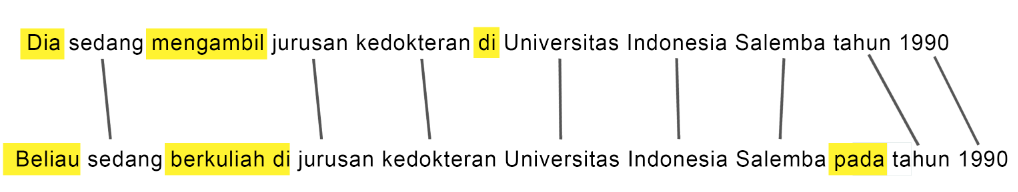
\includegraphics[width=0.9\linewidth]{pics/fitur_tambahan}
		\caption{Contoh penyesuaian kata antara 2 kalimat}
		\label{fig:fitur_tambahan}
	\end{figure}
	Berikut adalah perhitungan fitur tambahan untuk contoh \ref{fig:fitur_tambahan}.
	\begin{enumerate}
		\item Pasangan kelompok kata tidak bersesuaian yang tidak berpasangan dengan kelompok kosong adalah ([dia], [beliau]) dan ([mengambil], [berkuliah, di]). Maka, nilai fitur pertama adalah,
		\begin{equation}
		\frac{(similarity([dia], [beliau]) + similarity([mengambil], [berkuliah, di])}{2}
		\end{equation}
		\item Pasangan kelompok kata tidak bersesuaian yang berpasangan dengan kelompok kosong di T berjumlah satu, yaitu ([], [pada]). Sehingga nilai fitur kedua adalah \textit{sigmoid}(1).
		\item Pasangan kelompok kata tidak bersesuaian yang berpasangan dengan kelompok kosong di H berjumlah satu, yaitu ([di], []). Sehingga nilai fitur ketiga adalah \textit{sigmoid}(1).
		\item Ada delapan buah kata yang bersesuaian, sehingga nilai fitur keempat adalah,
		\begin{equation}
		(2 \times 8)/(11 + 12) = 0.59
		\end{equation}		
		\item Panjang LCSS dari contoh tersebut adalah tiga kata, sehingga nilai fitur kelima adalah,
		\begin{equation}
		(2 \times 3)/(11 + 12) = 0.26
		\end{equation}
		\item Kata pertama dari kedua kalimat tidak sama, sehingga nilai fitur keenam adalah 0.
	\end{enumerate}

	\subsection{Penentuan Classifier Kedua}
	\textit{Classifier} kedua dipilih dengan menggunakan percobaan 10-fold \textit{cross validation} terhadap fitur-fitur teks komentar pada data hasil anotasi manual. Ada beberapa kandidat \textit{classifier} yang akan digunakan, yaitu Neural Network (Multilayer Perceptron), Decision Tree, Naive Bayes, Multinomial Naive Bayes, dan Bayesian Network. 
	Ekstraksi fitur yang digunakan untuk \textit{view} kedua cukup sederhana, yaitu jumlah kemunculan N-gram tertentu pada teks komentar. Sebelum menentukan apa saja N-gram tersebut, teks komentar terlebih dahulu dianalisis berdasarkan frekuensi N-gram yang terdapat pada teks. Unigram, bigram, dan trigram yang paling sering muncul dijadikan sebagai fitur. Dengan cara tersebut, fitur yang didapat akan berjumlah banyak, namun tidak semua fitur baik untuk klasifikasi. Oleh karena itu, dilakukan pemilihan kombinasi atribut terbaik.